%lab report 2 of bresenhaum's line drawing algorithm and midpoint circle drawing algorithm in graphics.h
\documentclass[12pt]{article}

\usepackage{amsmath}
\usepackage{graphicx}
\usepackage[a4paper]{geometry}

\geometry{
  textwidth=\dimexpr\paperwidth-29mm,
  textheight=\dimexpr\paperheight-32mm,
  noheadfoot,
  nomarginpar
}

\setlength{\topskip}{0mm}
\setlength{\parindent}{0mm}

\begin{document}
	\title{Bresenham's Line Drawing Algorithm And Midpoint Circle Drawing Algorithm}
	\author{Jenish Pant}
	\date{\today}
	\maketitle

	\section{Objective}
	To implement Bresenham's Line Drawing Algorithm and Midpoint Circle Drawing Algorithm in graphics.h
	\section{Theory}
	\subsection{Bresenham's Line Drawing Algorithm}
	Bresenham's line algorithm is an algorithm that determines the points of an n-dimensional raster that should be selected in order to form a close approximation to a straight line between two points. It is commonly used to draw lines on a computer screen, as it uses only integer addition, subtraction and bit shifting, all of which are very cheap operations in standard computer architectures.
	It is an incremental error algorithm which improves on the DDA algorithm by using only integer calculations. Rather than performing one costly floating point multiplication, it performs two inexpensive integer multiplications and uses an integer decision variable to determine when to increment the y coordinate.\\
	\subsection{Midpoint Circle Drawing Algorithm}
	The midpoint circle algorithm is an algorithm used to determine the points needed for rasterizing a circle.
	It works by determining the points of an n-dimensional raster that best approximates a circle one pixel wide, where n is the dimension of the raster. It is an example of a first-order algorithm, as the error is related to the difference between the ideal circle and the rasterized circle. It is also an example of a group of algorithms known as midpoint circle algorithms, which all share the property that they are faster than naive implementations of the equation for a circle, $x^2 + y^2 = r^2$.\\
		

	\section{Algorithm}
	\subsection{Bresenham's Line Drawing Algorithm}
	\begin{enumerate}
		\item Input the two end points of the line, storing the left end point in $(x_0, y_0)$ 
		\item Plot the point $(x_0, y_0)$
		\item Calculate constants dx, dy, 2dy, and 2dy - 2dx, and obtain the starting value for the decision parameter as: $p_0 = 2dy - dx$.
		\item At each $x_k$ along the line, starting at k = 0, perform the following test:
		\begin{enumerate}
			\item If $p_k < 0$, the next point to plot is $(x_{k+1}, y_k)$ and,\\ $p_{k+1} = p_k + 2dy$.
			\item If $p_k \geq 0$ the next point to plot is $(x_{k+1}, y_{k+1})$ and,\\ $p_{k+1} = p_k + 2dy - 2dx$.
		\end{enumerate}
		\item Repeat step 4 dx times.
	\end{enumerate}

	\subsection{Midpoint Circle Drawing Algorithm}
	\begin{enumerate}
		\item Input the radius r and circle center $(x_c, y_c)$, and obtain the first point on the circumference of a circle centered on the origin as (0, r).
		\item Calculate the initial value of the decision parameter as $p_0 = 5/4 - r$.
		\item At each $x_k$ along the circumference, starting at k = 0, perform the following test:
		\begin{enumerate}
			\item If $p_k < 0$, the next point along the circle centered on (0,0) to plot is $(x_{k+1}, y_k)$ and,\\ $p_{k+1} = p_k + 2x_{k+1} + 1$.
			\item If $p_k \geq 0$, the next point to plot is $(x_{k+1}, y_{k-1})$ and,\\ $p_{k+1} = p_k + 2x_{k+1} - 2y_{k+1} + 1$.\\ \\
			where,\\
			$p_k = (x_k + 1)^2 + (y_k - 1/2)^2 - r^2$.\\
			$2x_{k+1} = 2x_k + 2$\\
			$2y_{k+1} = 2y_k - 2$
		\end{enumerate}
		\item Determine symmetry points in the other seven octants.
		\item Move each calculated point $(x, y)$ onto the circle centered on $(x_c, y_c)$, using the circle center coordinates in the translation equations $x = x + x_c$ and $y = y + y_c$.
		\item Repeat step 3 until x $\geq$ y.
	\end{enumerate}
	\section{Source Code}
	\subsection{Bresenham's Line Drawing Algorithm}
	\begin{verbatim}
	#include <stdio.h>
	#include <graphics.h>
	
	void drawLineBresenham() 
	{
	    int x1, y1, x2, y2;
	
	    printf("Enter the coordinates of the first point: ");
	    scanf("%d %d", &x1, &y1);
	    printf("Enter the coordinates of the second point: ");
	    scanf("%d %d", &x2, &y2);
	
	    int gd = DETECT, gm;
	    initgraph(&gd, &gm, "");
	
	    int dx = abs(x2 - x1), dy = abs(y2 - y1);
	    int slope  = 0;
	
	    if (dy > dx) 
	    {
	        slope = 1;
	        dy = dy + dx;
	        dx = dy - dx;
	        dy = dy - dx;
	    }
	
	    int p = 2 * dy - dx;
	    int twoDy = 2 * dy;
	    int twoDyMinusDx = 2 * (dy - dx);
	
	    int x, y;
	
	    if (x1 > x2)
	    {
	        x = x2;
	        y = y2;
	        x2 = x1;
	    }
	    else
	    {
	        x = x1;
	        y = y1;
	    }
	
	    putpixel(x, y, GREEN);
	
	    while (x < x2)
	    {
	        x++;
	        if (p < 0)
	            p += twoDy;
	        else
	        {
	            if (slope)
	                y++;
	            else
	                y += (y2 > y1) ? 1 : -1;
	            p += twoDyMinusDx;
	        }
	        putpixel(x, y, GREEN);
	    }
	
	    getch();
	    closegraph();
	}
		
	\end{verbatim}		

	\subsection{Midpoint Circle Drawing Algorithm}
	\begin{verbatim}
	
	#include <stdio.h>
	#include <graphics.h>
	
	void midpointCircle()
	{
	    int xc, yc, r;
	    printf("Enter the coordinates of the center: ");
	    scanf("%d %d", &xc, &yc);
	    printf("Enter the radius of the circle: ");
	    scanf("%d", &r);
	
	    int gd = DETECT, gm;
	    initgraph(&gd, &gm, "");
	
	    int x = 0;
	    int y = r;
	    int p = 1 - r;
	
	    // Plot the initial point in each quadrant
	    putpixel(x + xc, y + yc, GREEN);
	    putpixel(-x + xc, y + yc, GREEN);
	    putpixel(x + xc, -y + yc, GREEN);
	    putpixel(-x + xc, -y + yc, GREEN);
	
	    putpixel(y + xc, x + yc, GREEN);
	    putpixel(-y + xc, x + yc, GREEN);
	    putpixel(y + xc, -x + yc, GREEN);
	    putpixel(-y + xc, -x + yc, GREEN);
	
	    while (x++ < y)
	    {
	        if (p <= 0)
	        {
	            p = p + 2 * x + 1;
	        }
	        else
	        {
	            y--;
	            p = p + 2 * (x - y) + 1;
	        }
	
	        // All the perimeter points have already been printed
	        if (x > y) break;
	
	        // Printing the generated point and its reflection in the other octants
	        putpixel(x + xc, y + yc, GREEN);
	        putpixel(-x + xc, y + yc, GREEN);
	        putpixel(x + xc, -y + yc, GREEN);
	        putpixel(-x + xc, -y + yc, GREEN);
	
	        if (x != y)
	        {
	            putpixel(y + xc, x + yc, GREEN);
	            putpixel(-y + xc, x + yc, GREEN);
	            putpixel(y + xc, -x + yc, GREEN);
	            putpixel(-y + xc, -x + yc, GREEN);
	        }
	    }
	    getch();
	    closegraph();
	}
	\end{verbatim}
	
	\section{Output}

	\subsection{Bresenham's Line Drawing Algorithm And Midpoint Circle Drawing Algorithm}
	\begin{figure}[!h]
		%move to the left
		\hspace*{-1cm}
		\centering
		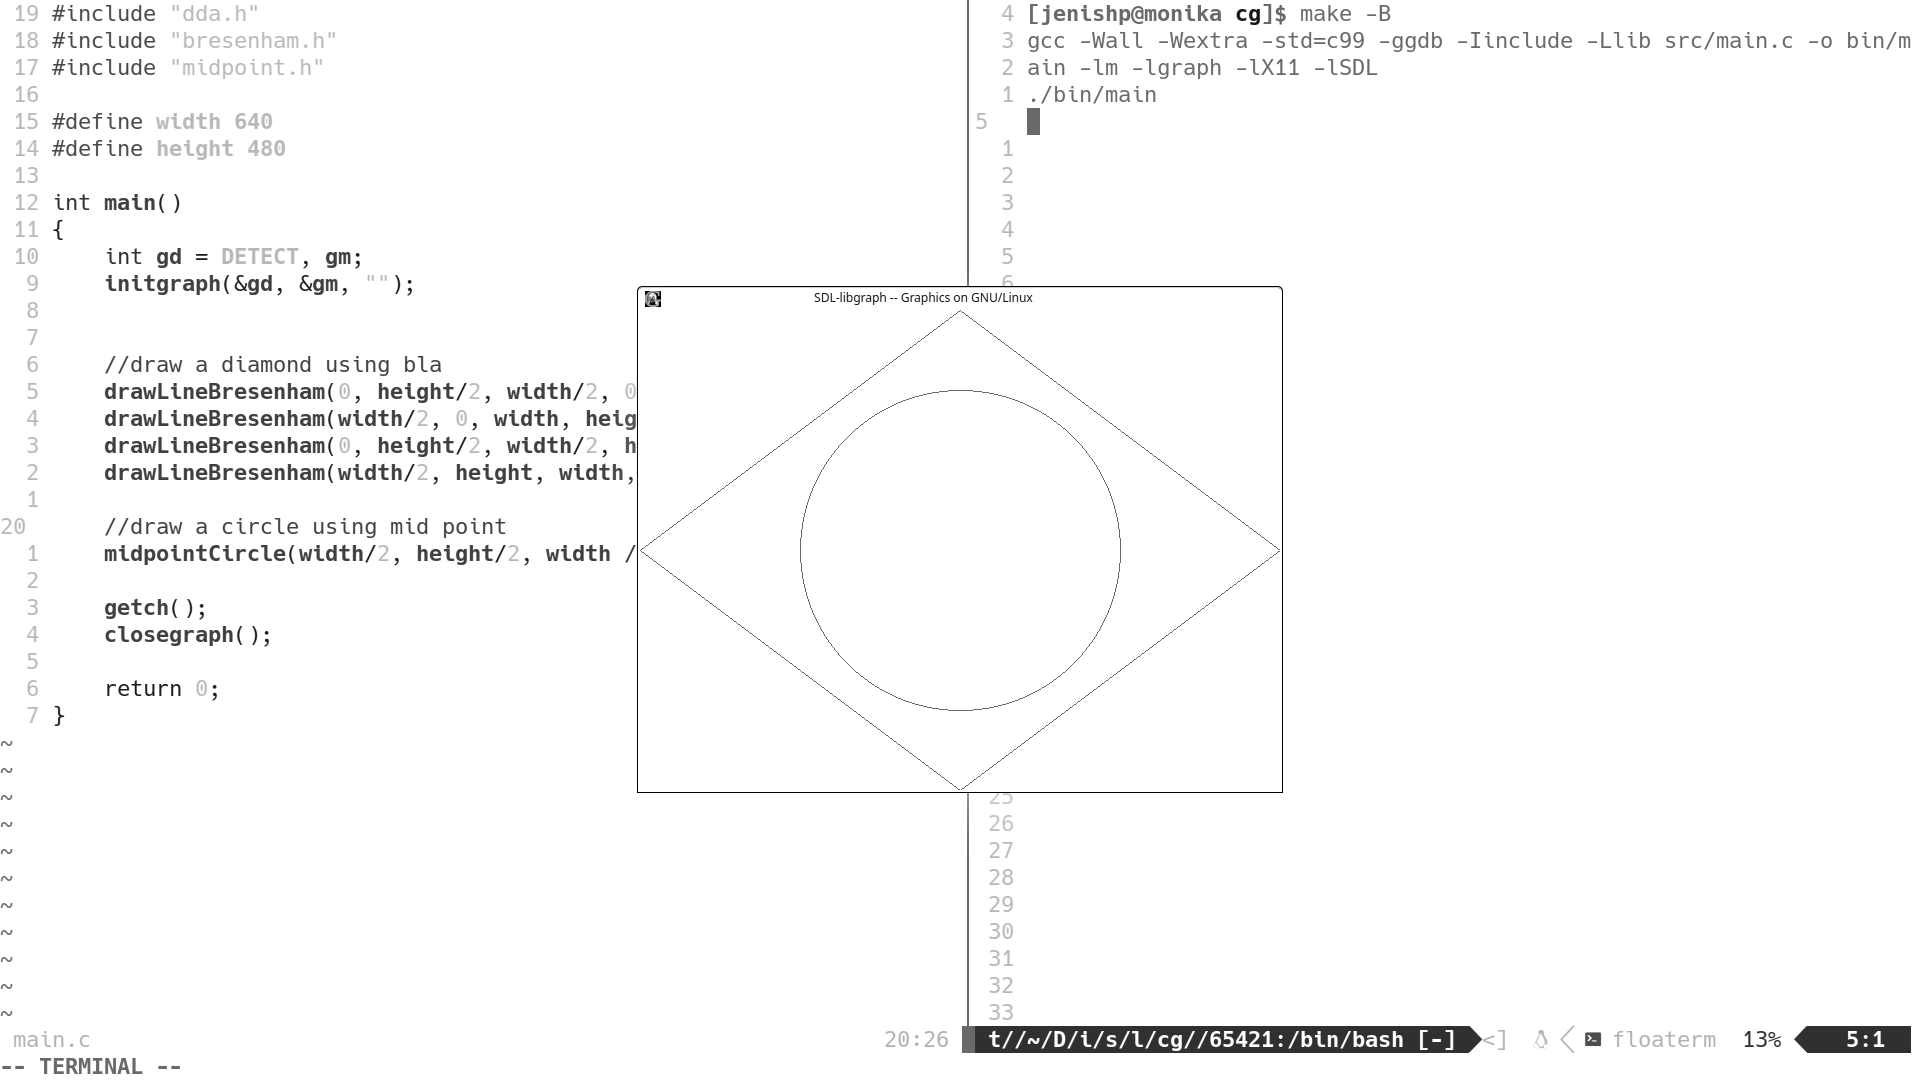
\includegraphics[width=1.01\linewidth]{output2.png}
		\caption{Bresenham's Line Drawing Algorithm And Midpoint Circle Drawing Algorithm in action}
		\label{fig:bresenham and circle}
	\end{figure}

	\section{Conclusion}
	We have implemented Bresenham's Line Drawing Algorithm and Midpoint Circle Drawing Algorithm in graphics.h
	BLA offers a significant speed improvement over DDA and other algorithms by using integer calculations instead of floating point.
	Midpoint circle algorithm is an efficient method of drawing circles in computer graphics. On modern computers it can be more efficient than trigonometric or approximating algorithm.
\end{document}

